\chapter{$B7kO@(B}

%$B4XO"O@J8(B\cite{sample}.

$B?^$N;2>H!"?^(B\ref{fig:yoshiki}

$BI=$N;2>H!"I=(B\ref{tab:sample}

\begin{figure}[hbt]
    \centering
    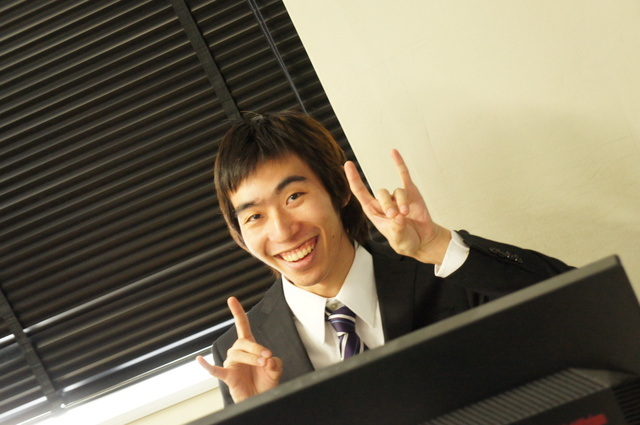
\includegraphics[scale=1.0,clip]{image/yoshiki_nico.jpg}
    \caption{Sample$B?^(B}
    \label{fig:yoshiki}
\end{figure}


\begin{table}[hbt]
    \caption{Sample$BI=(B}
    \centering
    \begin{tabular}{|c||c|c|c|c|c|}
        \hline
        & XXX & XX & XXXXX & XXXX & XXXX\\
        \hline\hline
        XXXX     & xxx & xxx & xxxx & xx & xx \\\hline
        XXXXX & xxx & xxx & xxxx & xx & xx \\\hline   
    \end{tabular}
    \label{tab:sample}
\end{table}






